\section{Architecture Overview}\label{architecture}

\subsection{Architecture of the SS ADCs}

The overall architecture of the SS ADCs is presented in Fig.~\ref{SSADC}. The main modules include column-parallel Correlated Double Sampling (CDS) circuits, comparators, 
and a column-shared ramp generator. Fig.~\ref{SSWAVE} shows the basic operational waveform of the SS ADCs. At the time when the ramp signal exceeds the output of a CDS circuit in a certain column, 
the corresponding comparator will be flipped and latch the time information $\Delta t$ in the 8-bit registers in that column as conversion results. 
And Such conversions across all columns will be done as soon as the ramp signal reaches $V_{refh}$.

\begin{figure}[htbp]
	\centerline{\includegraphics[width=3.5in]{./Figures/SSADC.eps}}
	\caption{Overall Architecture of the SS ADCs.}
	\label{SSADC}
\end{figure} 

\begin{figure}[htbp]
	\centerline{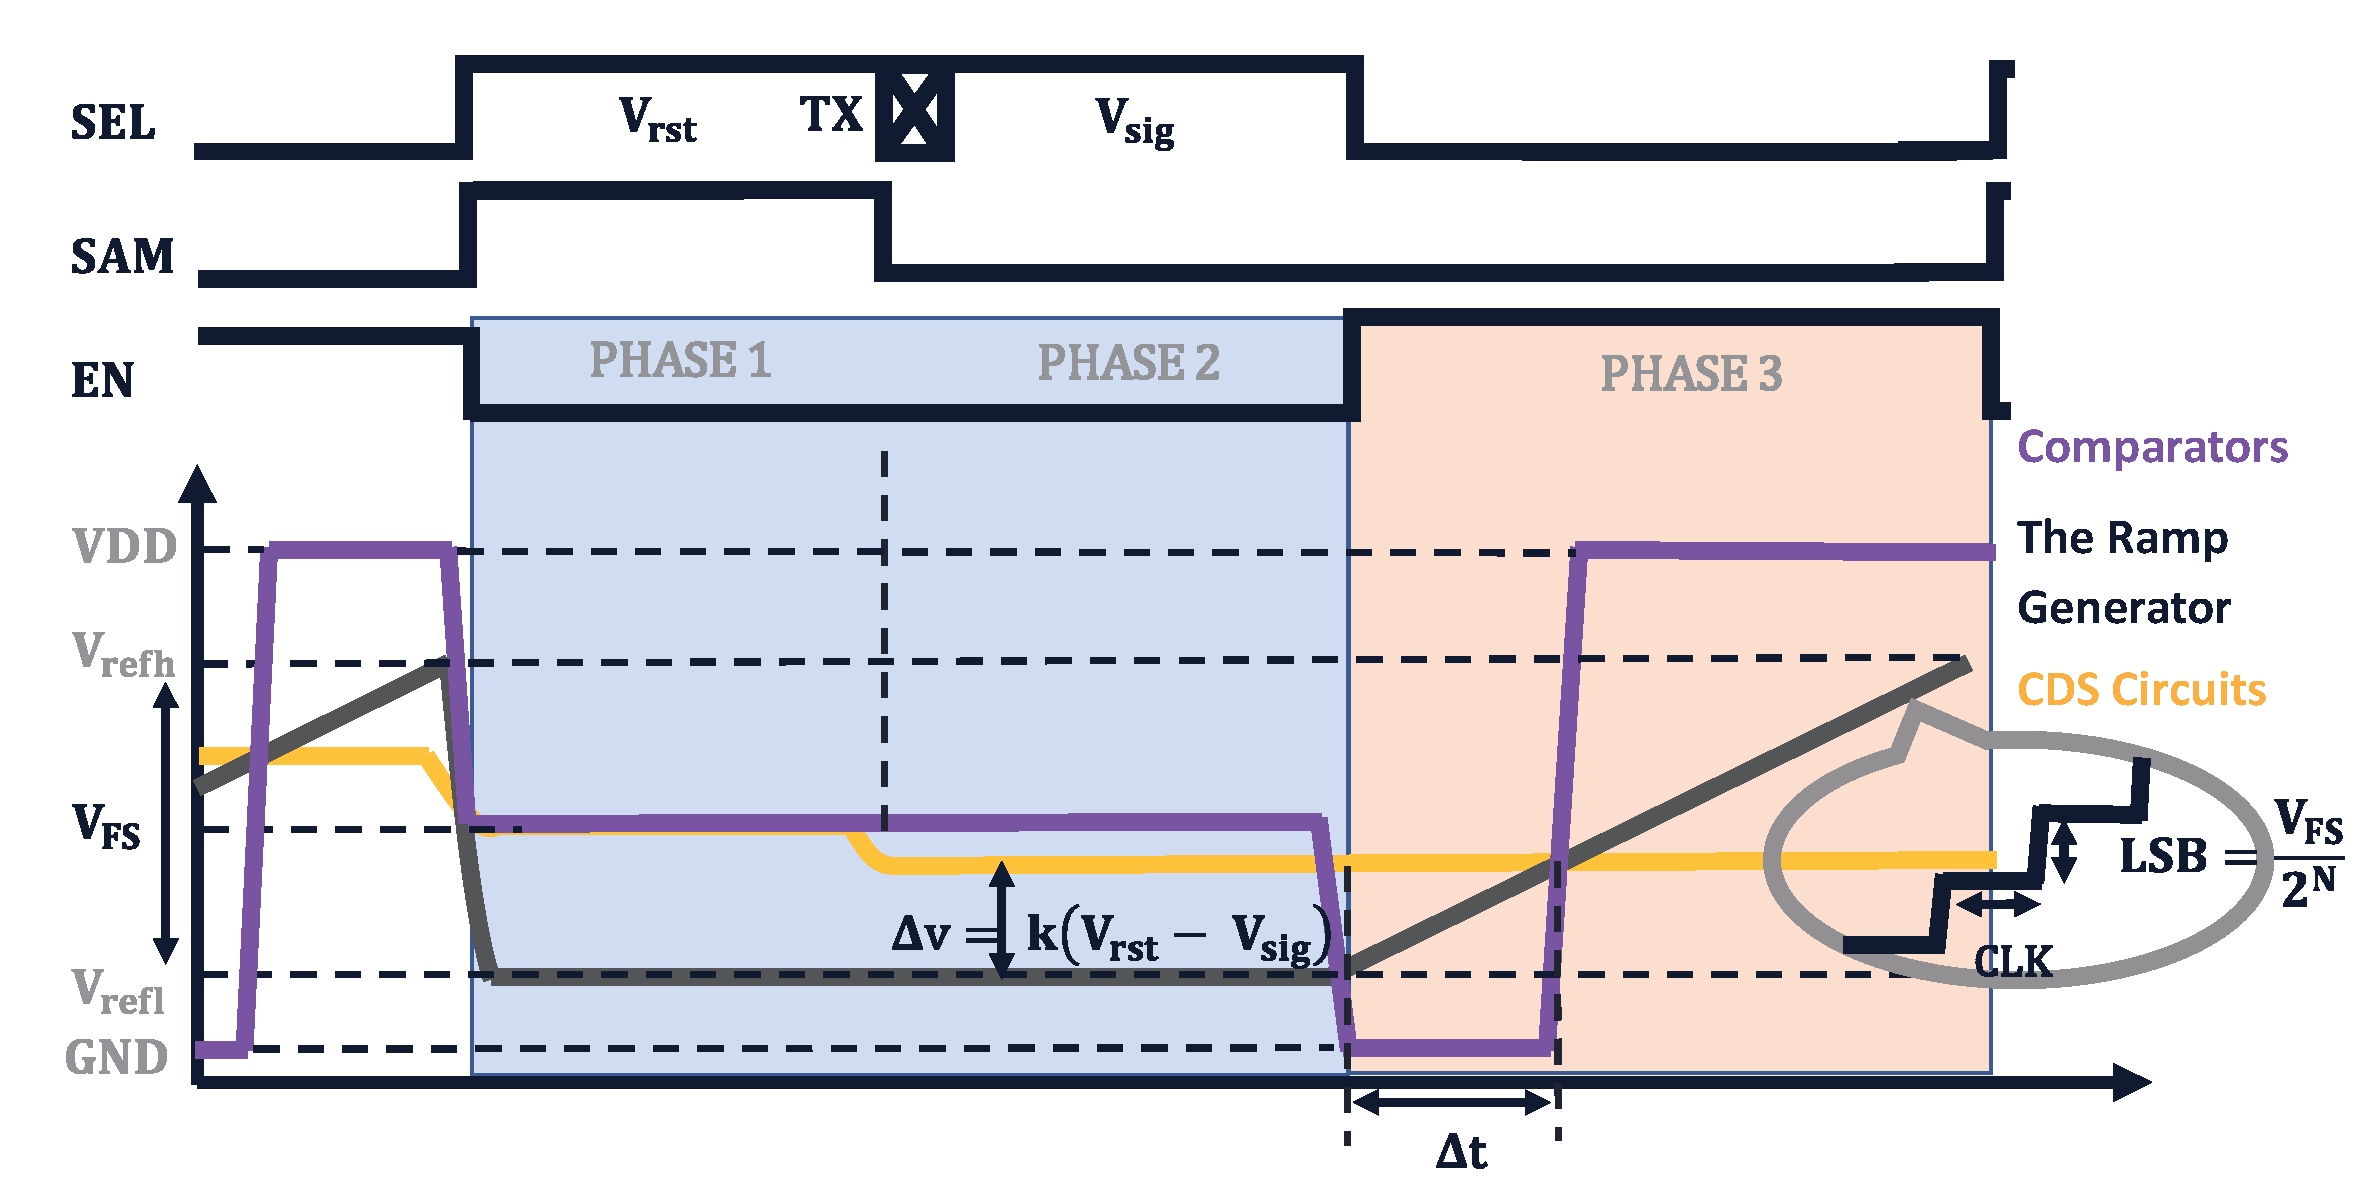
\includegraphics[width=3.5in]{./Figures/SSWAVE.eps}}
	\caption{Operational Waveform of the SS ADCs.}
	\label{SSWAVE}
\end{figure}

As the structure of the three main modules are described more specifically as follows, details of the three waves in Fig.~\ref{SSWAVE} are also revealed.

\subsubsection{CDS Circuits}

CDS circuits are the interface between the pixel array and the ADCs, responsible for subtracting the pixels’ signal voltages from reference voltages and 
amplifying the difference by a certain coefficient. The difference (i.e. $\Delta{V}$ in Fig.~\ref{SSWAVE}) is physically attached to the exposure time of the pixels, 
and the subtraction will help cancel the noises caused by the varying reference voltages. 

Switched-capacitor operational amplifiers are commonly used in CDS circuits as presented in Fig.~\ref{CDS}. According to the law of charge conservation, 
the output voltage of the CDS circuits (in PHASE2 of Fig.~\ref{SSWAVE}) can be calculated as \eqref{eq1}, consistent with the requirements. It is also noticed that the Input Offset Cancelation (IOS) is realized \cite{razavi_design_1992}, 
which is necessary because the amplifiers in different columns may have different offset voltage.

\begin{figure}[htbp]
	\centerline{\includegraphics[width=2.5in]{./Figures/CDS.eps}}
	\caption{the Structure of the CDS Circuits.}
	\label{CDS}
\end{figure} 

\begin{equation}
	\begin{aligned}
		V_{out}&=\left[ V_{ref}+\frac{C_1}{C_2}\ast\left(V_{rst}-V_{sig}\right)\right]\ast\frac{\beta A}{1+\beta A}\\
		&\;{+}\;\left(V\right._{refl}+V_{os})\ast\frac{A}{1+A}\ast\frac{1}{\beta A}\\
		&\;where\ \ \beta=\frac{C_2}{C_1+C_2}
		\label{eq1}
	\end{aligned}
\end{equation}

\subsubsection{the Ramp Generater}

As presented in Fig.~\ref{RAMP}, the ramp generator in the SS ADCs consists of a thermometer counter and a Capacitor Digital-to-Analog Converter (CDAC). 
While the capacitors in CDAC are being switched one by one from $V_{refl}$ to $V_{vefh}$, the output voltage of the ramp generator will be as \eqref{eq2} according to the law of charge conservation. 
In this equation, $N$ means the number of switched capacitors and $M$ means the total number of capacitors of the same size (for the 8-bit precision, the total number will be 255). 
Therefore, as in PHASE3 of Fig.~\ref{SSWAVE}, the ramp signal will be like stages from $V_{refl}$ to $V_{refh}$, of which the range matches with the output of CDS circuits. 
And the height of every stage is actually the Least Significant Bit (LSB) converted by the ADCs.

The three buffers in Fig.~\ref{RAMP} make sure that the reference voltages and ramp signal have enough driving capability, 
and the output buffer will be in the largest size because it has to drive hundreds of column-parallel comparators.

\begin{figure}[htbp]
	\centerline{\includegraphics[width=3.5in]{./Figures/RAMP.eps}}
	\caption{the Structure of the Ramp Generator in the SS ADCs.}
	\label{RAMP}
\end{figure} 

\begin{equation}
	V_{ramp}=V_{refl}+\frac{N}{M}\ast\left(V_{refh}-V_{refl}\right)
	\label{eq2}
\end{equation}

\subsubsection{Comparators}

The comparators work for comparing the CDS circuits' output and the ramp signal from the ramp generator. 
In the SS ADCs, two-stage open-loop comparators can be applied as presented in Fig.~\ref{COM}. Again according to the law of charge conservation, 
the comparators’ output (in PHASE3 of Fig.~\ref{SSWAVE}) can be calculated as \eqref{eq3}. The comparison will be dominated by $V_{ramp}-V_{cds}$ as long as the amplifiers’ open-loop gain 
is large enough while the IOS is also realized. In addition, the comparators’ speed relies on the amplifiers’ bandwidth and slew rate.

\begin{figure}[htbp]
	\centerline{\includegraphics[width=3.5in]{./Figures/COM.eps}}
	\caption{the Structure of the Comparators in the SS ADCs.}
	\label{COM}
\end{figure} 

\begin{equation}
	\begin{aligned}
		V_{out}&=A^2(V_{ramp}-V_{cds})\\
		&\;{+}\;\left(V_{refl}+V_{os}\right)\ast\frac{A}{1+A}\\ 		
		\label{eq3}
	\end{aligned}
\end{equation}

\subsection{Architecture of the SAR/SS ADCs}

The overall architecture of the SAR/SS ADCs is almost the same as the SS ADCs as presented in Fig.~\ref{SARADC}, and the only two differences are that the comparators are replaced by low-precision (4bit) SAR sub-ADCs and
the ramp generator is replaced by a Resistor Digital-to-Analog Converter (RDAC) with a one-hot counter.

As presented in Fig.~\ref{SAR}, a SAR sub-ADC is composed of two input buffers of the reference voltages, an array of digital-to-analog capacitors, a dynamical comparator and a module of SAR logic. While generating the upper 4-bit results, $V_{X}$ in the SAR sub-ADCs will be changed according to the SAR logic. That means after 4 comparisons 
with the reference voltage, $V_{X}$ will be as \eqref{eq4}, where $D_{U}\left[\,i\,\right]$ is the $i$ th bit of the upper 4 bits. 
And then the ramp generator will start working, making $V_{X}$ increase gradually as \eqref{eq5}, where $D_{L}\left[\,i\,\right]$ is the $i$ th bit of the lower 6 bits. 
At the time when $V_{X.2}$ exceeds $V_{ref}$, the corresponding $V_{cds}$ will be as \eqref{eq6}, which can be represented by the 10-bit conversion results, exactly.

It is worth noting that we assign 14 steps for the 4 comparisons with SAR logic. Both of the first and second comparison takes 4 steps and the following two comparison takes 3 steps. It is because that the more rapidly $V_{X}$ can be changed, the more time may required for comparison. As for the last comparison with SS logic, 1 step is enouph because $V_{X}$ will exceed $V_{ref}$ gradually, allowing the comparators to response in-time.

Fig.~\ref{RRAMP} shows the structure of the ramp generator in the SAR/SS ADCs, which consists of an R-string made up of 68 unit resistors. $V_{ramp}$ has a total number of 68 steps,
of which 64 steps with a step size of $(V_{refh}-V_{refl})/64$ are used to generate the lower 6-bit results and 4 redundant steps are used to make sure that the comparators 
will always be flipped to latch the results. In the working time, $V_{0}$ to $V_{67}$ in the ramp generator is sequentially selected as the input of the output buffer and thereby 
$V_{ramp}$ is changed from $V_{vefl}$ to $V_{vefl}+17/16(V_{refh}-V_{refl})$.

Compared to CDAC, RDAC is able to generate the ramp signal without the gain error caused by the input capacitors of the output buffer, 
which is necessary for achieving 10-bit precision in the SAR/SS mixed architecture.
Besides, the two buffers of the reference voltages in the RDAC require less energy than those in the CDAC due to less load capacitance.  

The related operational waveform of the SAR/SS ADCs is presented in Fig.~\ref{SARWAVE}. It is obvious that the upper 4-bit results (as the second last item of \eqref{eq6}) are generated 
with the SAR logic and the lower 6-bit results (as the last item of \eqref{eq6}) is counted according to the time between the ramp signal’s start and the comparators’ last flip.

\begin{figure}[htbp]
	\centerline{\includegraphics[width=3.5in]{./Figures/SARADC.eps}}
	\caption{Overall Architecture of the SAR/SS ADCs.}
	\label{SARADC}
\end{figure} 

\begin{figure}[htbp]
	\centerline{\includegraphics[width=3.5in]{./Figures/SAR.eps}}
	\caption{the Structure of the SAR Sub-ADCs in the SAR/SS ADCs.}
	\label{SAR}
\end{figure}

\begin{figure}[htbp] 
	\centerline{\includegraphics[width=3.5in]{./Figures/RRAMP.eps}}
	\caption{the Structure of the Ramp Generator in the SAR/SS ADCs.}
	\label{RRAMP}
\end{figure} 

\begin{equation}
	V_{X.1}=V_{cds}+\sum_{i=1}^{4} {\frac{V_{ref}}{2^{i}}\ast{D_{U}\left[\,i\,\right]}}
	\label{eq4}
\end{equation}

\begin{equation}
	\begin{aligned}
		&V_{X.2}=V_{X.1}+\frac{V_{ramp}}{2^4}\\ &where\  V_{ramp}=\frac{V_{ref}}{2^6-1}\ast\sum_{i=1}^{6}2^{6-i}\ast{D_{L}\left[\,i\,\right]}
		\label{eq5}
	\end{aligned}	
\end{equation}

\begin{equation}
	\begin{aligned}
		V_{cds}&=k\ast(V_{rst}-V_{sig})\\
		&\;{\approx}\;{V_{ref}-\sum_{i=1}^{4} \frac{V_{ref}}{2^{i}}\ast{D_{U}\left[\,i\,\right]}-\sum_{i=1}^{6} \frac{V_{ref}}{2^{4+i}}\ast{D_{L}\left[\,i\,\right]}}
		\label{eq6}
	\end{aligned}
\end{equation}

\begin{figure}[htbp]
	\centerline{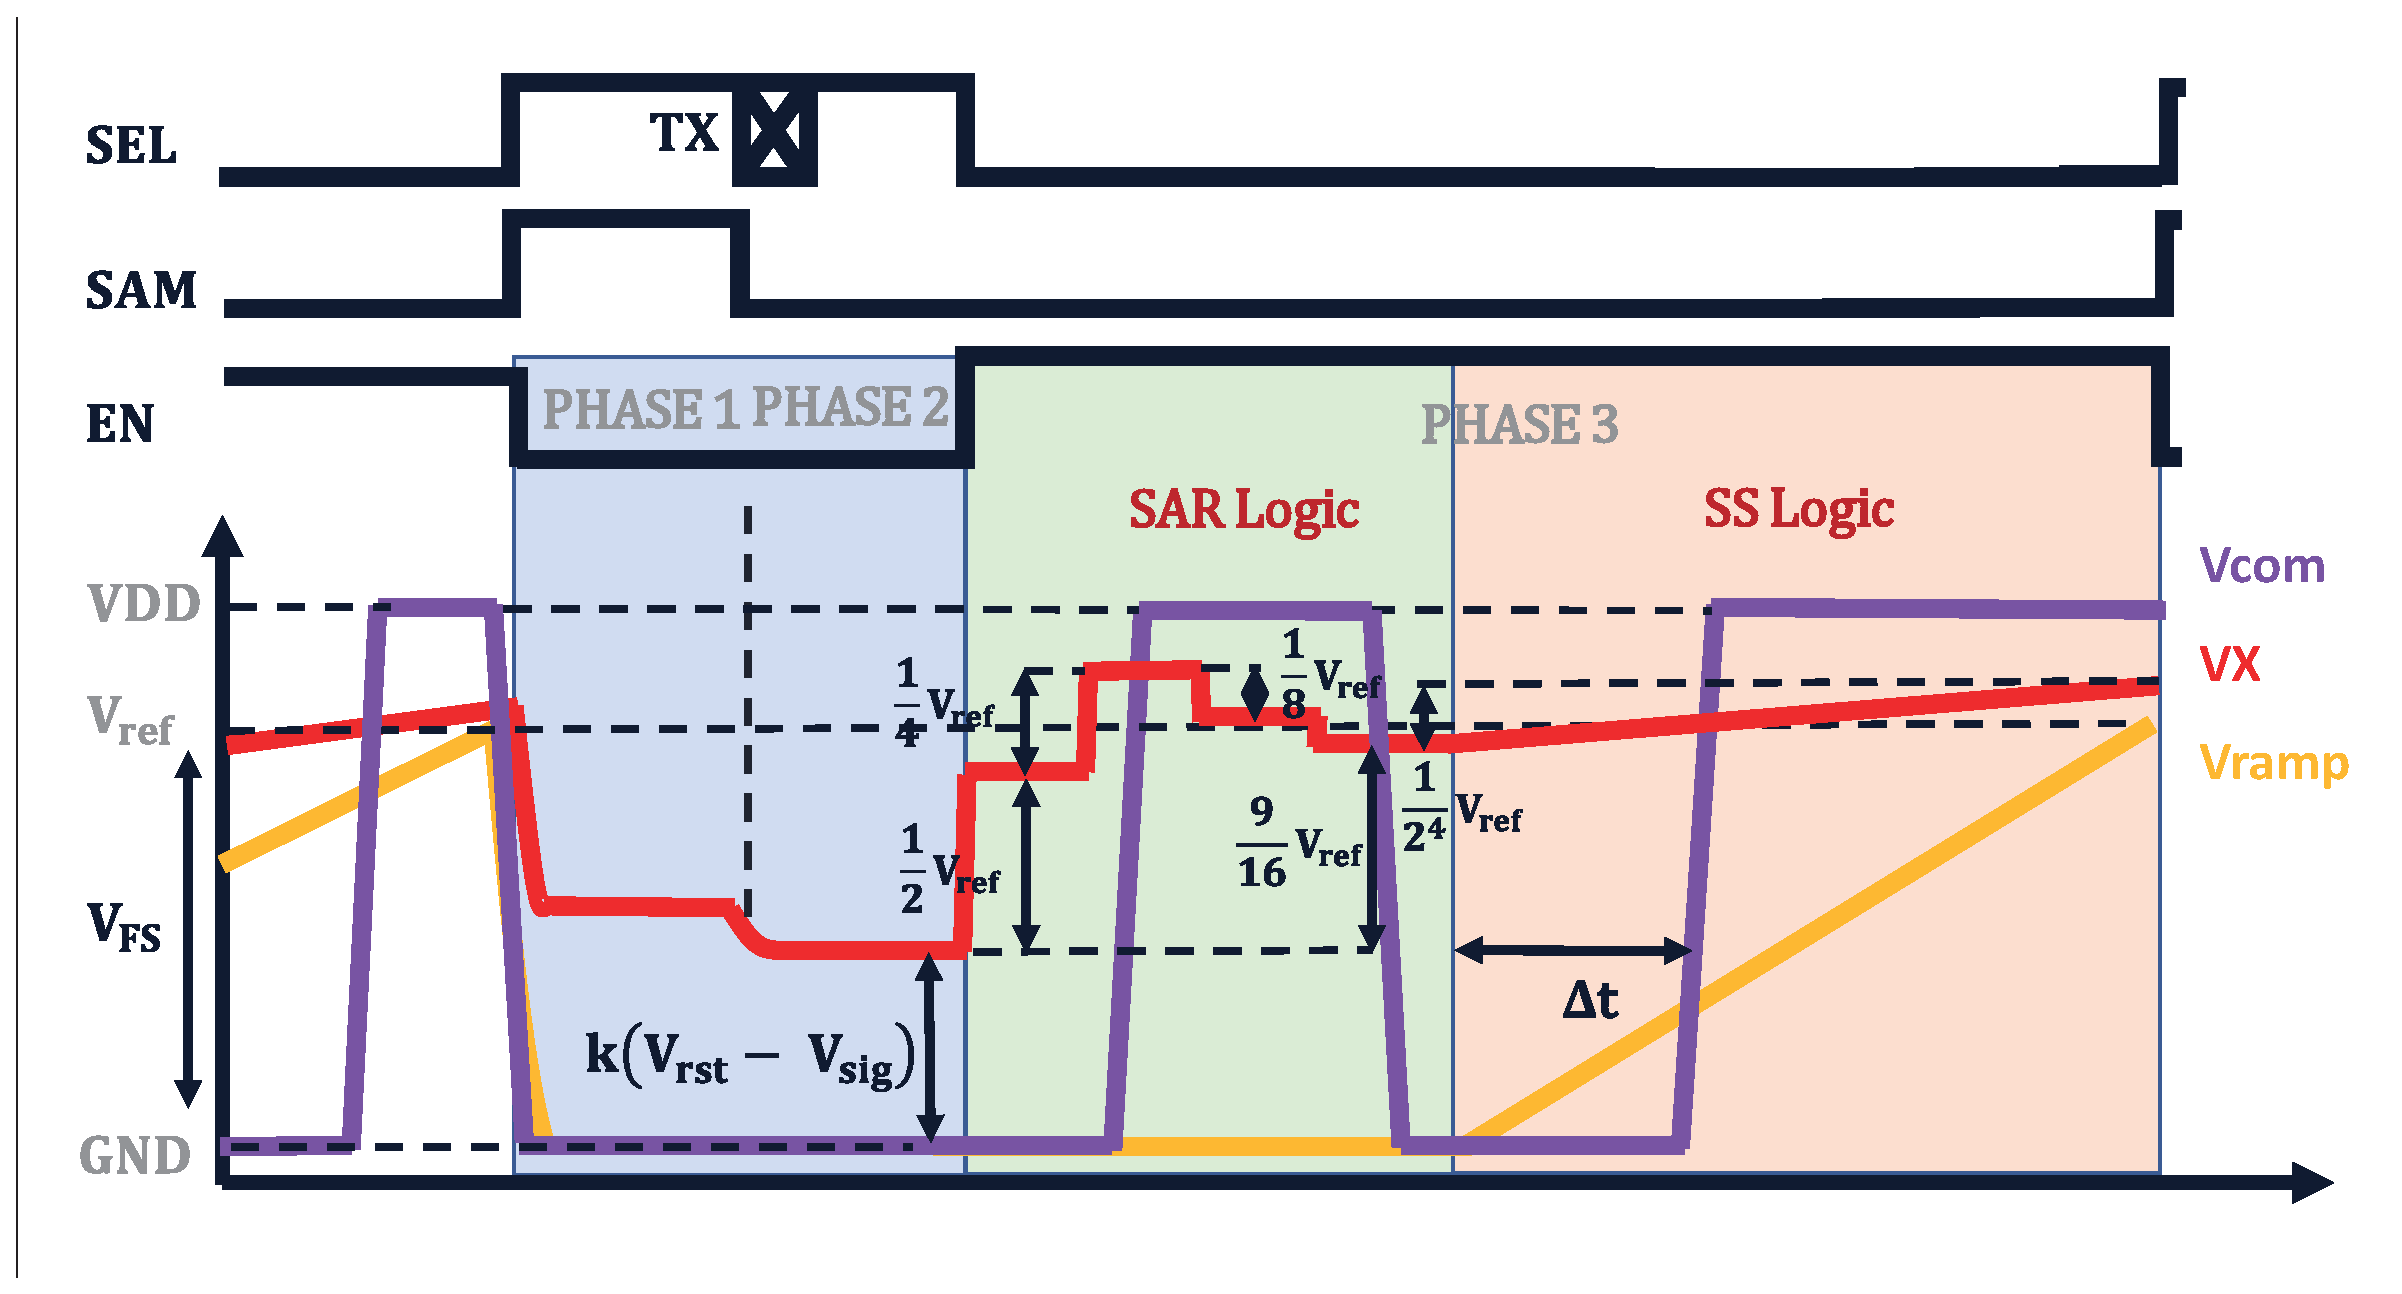
\includegraphics[width=3.5in]{./Figures/SARWAVE.eps}}
	\caption{Operational Waveform of the SAR/SS ADCs.}
	\label{SARWAVE}
\end{figure} 

As for the dynamical comparators inside the SAR sub-ADCs, traditional structure of a strong-arm comparator with pre-amplifiers is adopted as presented in Fig.~\ref{LATCH}. Such comparators 
are suitable for multiple comparisons because high speed is easy to achieve. Besides, the pre-amps’ offset voltages can be canceled effectively through the Output Offset Cancelation (OOS) \cite{razavi_design_1992}.

\begin{figure}[htbp]
	\centerline{\includegraphics[width=3.5in]{./Figures/LATCH.eps}}
	\caption{the Structure of the Comparators in the SAR Sub-ADCs.}
	\label{LATCH}
\end{figure} 

The reasons why we choose 4/8-bit adaptive-precision for the SS ADCs and 4/10-bit adaptive-precision for the SAR/SS ADCs are discussed in Sect.~\ref{discussion}.
